% questions.tex —— 2005 年·春季北京卷·理科 · 题目内容片段（无答案）
% 由 tools/generate_projects.py 依来源总账自 2005/2005_数学真题_春季北京理_试题.md 生成，勿手改（改源 MD 后重跑）


\begin{gktip}
\textbf{来源说明}：题签、题面和页脚页码依据固定 PDF 春季高考/2005/2005春季北京理.pdf 转录。文件 SHA-256 与来源清单一致，PDF 共 2 页 A3 横向，页脚页码为 213–214；对应上游 Git blob 为 ec69672989a921864315ba57d7debe044e492705。此副本已按固定字节绑定为 gk-2005-spring-beijing-science；该绑定只标识本库采用的文件，不认证发布者、版次或来源链。

\textbf{转录说明}：原生文字层仅辅助定位和核字；两页均按整页图像逐页目视转录，并由主会话对照源页复核。题面共 20 题：第 1–8 题选择，第 9–14 题填空，第 15–20 题解答。PDF 只含题面，本文不补写答案、解析或分值。

\textbf{图形说明}：第 2、12、16、18 题的原卷图已按拓扑与线型重绘为 TikZ；相对位置仅作示意，详见图表清单。
\end{gktip}

\gkpart{一、选择题}

\begin{question}
\gkti{1}

i $-$ 2 的共轭复数是（ ）

（A）2 + i　　（B）2 $-$ i　　（C）$-$2 + i　　（D）$-$2 $-$ i

\Needspace{0.4\textheight}
\end{question}
\begin{question}
\gkti{2}

函数 $y=|\log_2 x|$ 的图象是（ ）
\nopagebreak[4]
\begin{center}% Source-page vector redraw of the four function-graph options.
% Curves preserve visible topology only; coordinates are schematic.
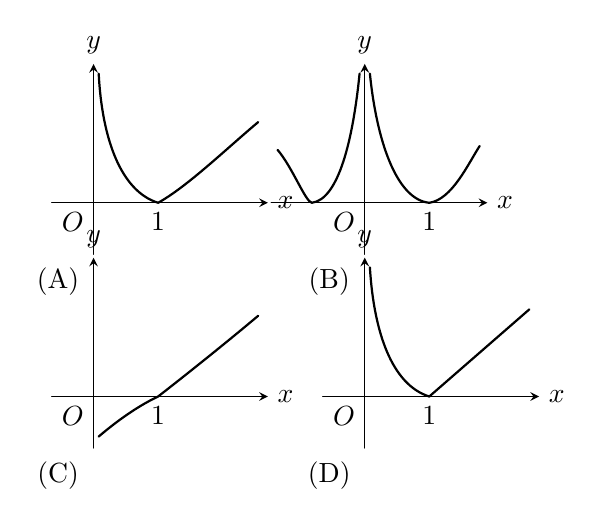
\begin{tikzpicture}[>=stealth, line cap=round, line join=round, scale=.82]
% Option A
\begin{scope}[shift={(0,0)}]
  \draw[->] (-.65,0)--(2.7,0) node[right] {$x$}; \draw[->] (0,-.8)--(0,2.15) node[above] {$y$};
  \node[below left] at (0,0) {$O$}; \node[below] at (1,0) {$1$}; \node at (-.55,-1.22) {(A)};
  \draw[thick] (.08,2.0) .. controls (.13,1.0) and (.42,.18) .. (1,0) .. controls (1.45,.25) and (2.05,.83) .. (2.55,1.25);
\end{scope}
% Option B
\begin{scope}[shift={(4.2,0)}]
  \draw[->] (-1.45,0)--(1.9,0) node[right] {$x$}; \draw[->] (0,-.8)--(0,2.15) node[above] {$y$};
  \node[below left] at (0,0) {$O$}; \node[below] at (1,0) {$1$}; \node at (-.55,-1.22) {(B)};
  \draw[thick] (-1.35,.82) .. controls (-1.12,.55) and (-.92,.02) .. (-.82,0) .. controls (-.4,.05) and (-.18,1.0) .. (-.08,2.0);
  \draw[thick] (.08,2.0) .. controls (.18,1.0) and (.48,.05) .. (1,0) .. controls (1.35,.05) and (1.6,.6) .. (1.78,.88);
\end{scope}
% Option C
\begin{scope}[shift={(0,-3.0)}]
  \draw[->] (-.65,0)--(2.7,0) node[right] {$x$}; \draw[->] (0,-.8)--(0,2.15) node[above] {$y$};
  \node[below left] at (0,0) {$O$}; \node[below] at (1,0) {$1$}; \node at (-.55,-1.22) {(C)};
  \draw[thick] (.08,-.62) .. controls (.28,-.45) and (.62,-.18) .. (1,0) .. controls (1.45,.35) and (2.05,.83) .. (2.55,1.25);
\end{scope}
% Option D
\begin{scope}[shift={(4.2,-3.0)}]
  \draw[->] (-.65,0)--(2.7,0) node[right] {$x$}; \draw[->] (0,-.8)--(0,2.15) node[above] {$y$};
  \node[below left] at (0,0) {$O$}; \node[below] at (1,0) {$1$}; \node at (-.55,-1.22) {(D)};
  \draw[thick] (.08,2.0) .. controls (.14,1.0) and (.42,.18) .. (1,0);
  \draw[thick] (1,0)--(2.55,1.35);
\end{scope}
\end{tikzpicture}
\end{center}
\nopagebreak[4]
\end{question}
\begin{question}
\gkti{3}

有如下三个命题：

① 分别在两个平面内的两条直线一定是异面直线；<br>
② 垂直于同一个平面的两条直线是平行直线；<br>
③ 过平面 $\alpha$ 的一条斜线有一个平面与平面 $\alpha$ 垂直。

其中正确命题的个数为（ ）

（A）0　　（B）1　　（C）2　　（D）3

\end{question}
\begin{question}
\gkti{4}

如果函数 $f(x)=\sin(\pi x+\theta)$（$0<\theta<2\pi$）的最小正周期是 $T$，且当 $x=2$ 时取得最大值，那么（ ）

（A）$T=2,\ \theta=\dfrac{\pi}{2}$　　（B）$T=1,\ \theta=\pi$<br>
（C）$T=2,\ \theta=\pi$　　（D）$T=1,\ \theta=\dfrac{\pi}{2}$

\end{question}
\begin{question}
\gkti{5}

设 $abc\ne 0$，“$ac>0$”是“曲线 $ax^2+by^2=c$ 为椭圆”的（ ）

（A）充分非必要条件　　（B）必要非充分条件<br>
（C）充分必要条件　　（D）既非充分又非必要条件

\end{question}
\begin{question}
\gkti{6}

已知双曲线的两个焦点为 $F_1(-\sqrt5,0),\ F_2(\sqrt5,0)$，$P$ 是此双曲线上的一点，且 $PF_1\perp PF_2$，$|PF_1|\cdot|PF_2|=2$，则该双曲线的方程是（ ）

（A）$\dfrac{x^2}{2}-\dfrac{y^2}{3}=1$　　（B）$\dfrac{x^2}{3}-\dfrac{y^2}{2}=1$<br>
（C）$\dfrac{x^2}{4}-y^2=1$　　（D）$x^2-\dfrac{y^2}{4}=1$

\end{question}
\begin{question}
\gkti{7}

在 $\triangle ABC$ 中，已知 $2\sin A\cos B=\sin C$，那么 $\triangle ABC$ 一定是（ ）

（A）直角三角形　　（B）等腰三角形<br>
（C）等腰直角三角形　　（D）正三角形

\end{question}
\begin{question}
\gkti{8}

若不等式 $(-1)^n a<2+\dfrac{(-1)^{n+1}}{n}$ 对于任意正整数 $n$ 恒成立，则实数 $a$ 的取值范围是（ ）

（A）$\left[-2,\dfrac32\right)$　　（B）$\left(-2,\dfrac32\right)$<br>
（C）$\left[-3,\dfrac32\right)$　　（D）$\left(-3,\dfrac32\right)$

\end{question}
\gkpart{二、填空题}

\begin{question}
\gkti{9}

$\displaystyle\lim_{n\to\infty}\frac{n^2+2n}{2n^2-3}=$ \gkblank{}.

\end{question}
\begin{question}
\gkti{10}

已知 $\sin\dfrac\theta2+\cos\dfrac\theta2=\dfrac{2\sqrt3}{3}$，那么 $\sin\theta$ 的值为 \gkblank{}，$\cos2\theta$ 的值为 \gkblank{}。

\end{question}
\begin{question}
\gkti{11}

若圆 $x^2+y^2+mx-\dfrac14=0$ 与直线 $y=-1$ 相切，且其圆心在 $y$ 轴的左侧，则 $m$ 的值为 \gkblank{}.

\Needspace{0.4\textheight}
\end{question}
\begin{question}
\gkti{12}

如图，正方体 $ABCD-A_1B_1C_1D_1$ 的棱长为 $a$，将该正方体沿对角面 $BB_1D_1D$ 切成两块，再将这两块拼接成一个不是正方体的四棱柱，那么所得四棱柱的全面积为 \gkblank{}.
\nopagebreak[4]
\begin{center}% Source-page vector redraw from 2005 Spring Beijing Science, printed p. 213, Q12.
% Kept as a separate source-specific file. Dashed edges follow the visible source line styles.
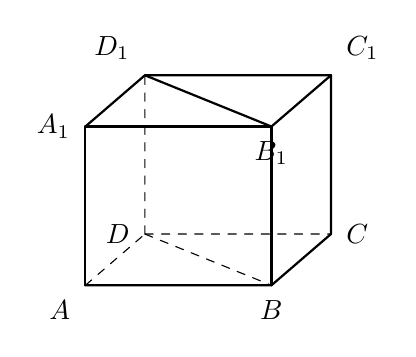
\begin{tikzpicture}[line cap=round, line join=round, scale=1.05]
\coordinate (A) at (0,0); \coordinate (B) at (2.25,0);
\coordinate (D) at (.72,.62); \coordinate (C) at (2.97,.62);
\coordinate (A1) at (0,1.92); \coordinate (B1) at (2.25,1.92);
\coordinate (D1) at (.72,2.54); \coordinate (C1) at (2.97,2.54);
% Solid visible cube edges
\draw[thick] (A)--(B)--(C);
\draw[thick] (A)--(A1)--(B1)--(B);
\draw[thick] (B1)--(C1)--(C);
\draw[thick] (A1)--(D1)--(C1);
\draw[thick] (C)--(C1);
% Hidden cube edges and hidden diagonal of BB1D1D
\draw[dashed] (A)--(D) (D)--(C) (D)--(D1);
\draw[dashed] (D)--(B);
% Visible diagonal of BB1D1D
\draw[thick] (D1)--(B1);
\node[below left=2pt] at (A) {$A$};
\node[below=2pt] at (B) {$B$};
\node[right=2pt] at (C) {$C$};
\node[left=2pt] at (D) {$D$};
\node[left=2pt] at (A1) {$A_1$};
\node[below=2pt] at (B1) {$B_1$};
\node[above left=2pt] at (D1) {$D_1$};
\node[above right=2pt] at (C1) {$C_1$};
\end{tikzpicture}
\end{center}
\nopagebreak[4]
\end{question}
\begin{question}
\gkti{13}

从 $-1,\ 0,\ 1,\ 2$ 这四个数中选三个不同的数作为函数 $f(x)=ax^2+bx+c$ 的系数，可组成不同的二次函数共有 \gkblank{} 个，其中不同的偶函数共有 \gkblank{} 个。（用数字作答）

\end{question}
\begin{question}
\gkti{14}

若关于 $x$ 的不等式 $x^2-ax-a>0$ 的解集为 $(-\infty,+\infty)$，则实数 $a$ 的取值范围是 \gkblank{}；若关于 $x$ 的不等式 $x^2-ax-a\leqslant-3$ 的解集不是空集，则实数 $a$ 的取值范围是 \gkblank{}.

\end{question}
\gkpart{三、解答题}

\begin{question}
\gkti{15}

设函数 $f(x)=\lg(2x-3)$ 的定义域为集合 $M$，函数 $g(x)=\sqrt{1-\dfrac2{x-1}}$ 的定义域为集合 $N$。求：

（1） 集合 $M,\ N$；<br>
（2） 集合 $M\cap N,\ M\cup N$。

\Needspace{0.4\textheight}
\end{question}
\begin{question}
\gkti{16}

如图，正三角形 $ABC$ 的边长为 $3$，过其中心 $G$ 作 $BC$ 边的平行线，分别交 $AB\text{、}AC$ 于 $B_1\text{、}C_1$. 将 $\triangle AB_1C_1$ 沿 $B_1C_1$ 折起到 $\triangle A_1B_1C_1$ 的位置，使点 $A_1$ 在平面 $BB_1C_1C$ 上的射影恰是线段 $BC$ 的中点 $M$. 求：

（1） 二面角 $A_1-B_1C_1-M$ 的大小；<br>
（2） 异面直线 $A_1B_1$ 与 $CC_1$ 所成角的大小.（用反三角函数表示）
\nopagebreak[4]
\begin{center}% Source-page vector redraw from 2005 Spring Beijing Science, printed p. 213, Q16.
% Schematic perspective only. Dashed segments are the source's obscured original triangle edges.
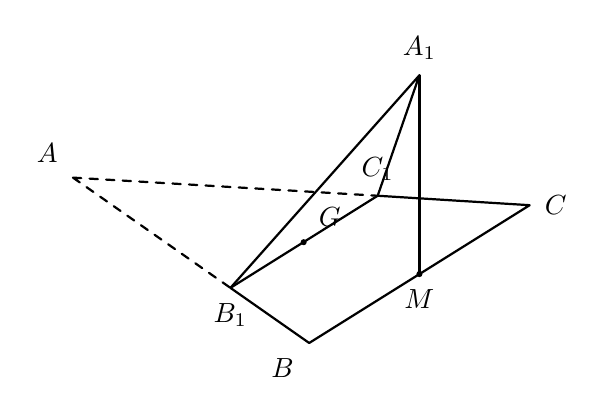
\begin{tikzpicture}[line cap=round, line join=round, scale=1.0]
\coordinate (A) at (-2,.90); \coordinate (B) at (1,-1.20); \coordinate (C) at (3.8,.55);
\coordinate (B1) at (0,-.50); \coordinate (C1) at (1.87,.67);
\coordinate (G) at (.93,.08); \coordinate (M) at (2.4,-.325); \coordinate (A1) at (2.4,2.2);
% Original triangle portions, folded triangle, and crease
\draw[dashed, thick] (A)--(B1) (A)--(C1);
\draw[thick] (B1)--(B)--(C)--(C1)--cycle;
\draw[thick] (A1)--(B1) (A1)--(C1);
% Median/projection line and named points on the crease/base
\draw[thick] (A1)--(M);
\fill (G) circle (1.1pt) (M) circle (1.1pt);
\node[above left=2pt] at (A) {$A$};
\node[below left=2pt] at (B) {$B$};
\node[right=2pt] at (C) {$C$};
\node[below=2pt] at (B1) {$B_1$};
\node[above=2pt] at (C1) {$C_1$};
\node[above right=2pt] at (G) {$G$};
\node[above=2pt] at (A1) {$A_1$};
\node[below=2pt] at (M) {$M$};
\end{tikzpicture}
\end{center}
\nopagebreak[4]
\end{question}
\begin{question}
\gkti{17}

已知 $\{a_n\}$ 是等比数列，$a_1=2,\ a_3=18$；$\{b_n\}$ 是等差数列，$b_1=2$，$b_1+b_2+b_3+b_4=a_1+a_2+a_3>20$。

（1） 求数列 $\{b_n\}$ 的通项公式；<br>
（2） 求数列 $\{b_n\}$ 的前 $n$ 项和 $S_n$ 的公式；<br>
（3） 设 $P_n=b_1+b_4+b_7+\cdots+b_{3n-2},\ Q_n=b_{10}+b_{12}+b_{14}+\cdots+b_{2n+8}$，其中 $n=1,2,\cdots$，试比较 $P_n$ 与 $Q_n$ 的大小，并证明你的结论。

\Needspace{0.4\textheight}
\end{question}
\begin{question}
\gkti{18}

如图，$O$ 为坐标原点，直线 $l$ 在 $x$ 轴和 $y$ 轴上的截距分别是 $a$ 和 $b$，且交抛物线 $y^2=2px$（$p>0$）于 $M(x_1,y_1)\text{、}N(x_2,y_2)$ 两点。

（1） 写出直线 $l$ 的截距式方程；<br>
（2） 证明：$\dfrac1{y_1}+\dfrac1{y_2}=\dfrac1b$；<br>
（3） 当 $a=2p$ 时，求 $\angle MON$ 的大小.
\nopagebreak[4]
\begin{center}% Source-page vector redraw from 2005 Spring Beijing Science, printed p. 214, Q18.
% The normalized curve and line illustrate only the source-visible topology; no parameters are inferred.
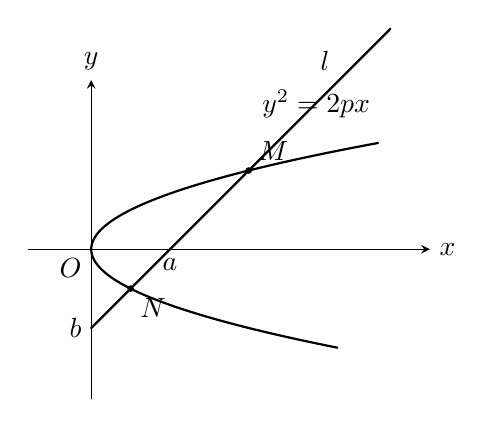
\begin{tikzpicture}[>=stealth, line cap=round, line join=round, scale=1.0]
\draw[->] (-.8,0)--(4.3,0) node[right] {$x$};
\draw[->] (0,-1.9)--(0,2.15) node[above] {$y$};
\node[below left] at (0,0) {$O$};
\draw[thick, domain=-1.25:1.35, samples=100, variable=\t]
  plot ({2*\t*\t},{\t});
% Schematic secant: it crosses y-axis below O and x-axis to the right of O.
\draw[thick] (0,-1)--(3.8,2.8);
\coordinate (M) at (2,1); \coordinate (N) at (.5,-.5);
\fill (M) circle (1.2pt) (N) circle (1.2pt);
\node[above right] at (M) {$M$}; \node[below right] at (N) {$N$};
\node[below] at (1,0) {$a$}; \node[left] at (0,-1) {$b$};
\node[above right] at (2.05,1.55) {$y^2=2px$};
\node[above left] at (3.15,2.15) {$l$};
\end{tikzpicture}
\end{center}
\nopagebreak[4]
\end{question}
\begin{question}
\gkti{19}

经过长期观测得到：在交通繁忙的时段内，某公路段汽车的车流量 $y$（千辆/小时）与汽车的平均速度 $v$（千米/小时）之间的函数关系为：

$\displaystyle y=\frac{920v}{v^2+3v+1600}\quad(v>0)$。

（1） 在该时段内，当汽车的平均速度 $v$ 为多少时，车流量最大？最大车流量为多少？（精确到 $0.1$ 千辆/小时）<br>
（2） 若要求在该时段内车流量超过 $10$ 千辆/小时，则汽车站的平均速度应在什么范围内？

\end{question}
\begin{question}
\gkti{20}

现有一组互不相同且从小到大排列的数据：$a_0,\ a_1,\ a_2,\ a_3,\ a_4,\ a_5$，其中 $a_0=0$。为提取反映数据间差异程度的某种指标，今对其进行如下加工：记

$T=a_0+a_1+\cdots+a_5,\quad x_n=\dfrac n5,\quad y_n=\dfrac1T(a_0+a_1+\cdots+a_n)$，作函数 $y=f(x)$，使其图象为逐点依次连接点 $P_n(x_n,y_n)$（$n=0,1,2,\cdots,5$）的折线。

（1） 求 $f(0)$ 和 $f(1)$ 的值；<br>
（2） 设 $P_{n-1}P_n$ 的斜率为 $k_n$（$n=1,2,3,4,5$），判断 $k_1,\ k_2,\ k_3,\ k_4,\ k_5$ 的大小关系；<br>
（3） 证明：当 $x\in(0,1)$ 时，$f(x)<x$；<br>
（4） 求由函数 $y=x$ 与 $y=f(x)$ 的图象所围成图形的面积。（用 $a_1,\ a_2,\ a_3,\ a_4,\ a_5$ 表示）

\end{question}